\documentclass[a4paper,12pt]{article}
\usepackage[utf8]{inputenc}
\usepackage{graphicx}
\usepackage{amsmath}
\usepackage{amssymb}
\usepackage{hyperref}
\usepackage{caption}
\usepackage{subcaption}

\newcommand{\mb}[1]{\ensuremath{\mathbf{#1}}}
\newcommand{\mc}[1]{\ensuremath{\mathcal{#1}}}
\newcommand{\mbb}[1]{\ensuremath{\mathbb{#1}}}

%opening
\title{Solution of the third exercise assignment}
\author{Lucas Nogueira Ribeiro}
\date{}

\begin{document}

\maketitle

The Python source code written to solve this assignment is available at \url{https://github.com/lnribeiro/patternrecognition}.

\subsection*{Exercise \#01}

\paragraph{First covariance matrix} The first covariance matrix \verb|C_I| and its partitions \verb|Caa, Cbb, Cab, Cba| are given by:
\begin{verbatim}
C_I:
[[ 4.  0.  0.]
 [ 0.  4.  0.]
 [ 0.  0.  4.]]

Caa:
[[ 4.  0.]
 [ 0.  4.]]
 
Cbb:
4.0

Cab:
[[ 0.]
 [ 0.]]
 
Cba:
[[ 0.  0.]]
\end{verbatim}
The precision matrix \verb|P_I| and its partitions \verb|Paa, Pbb, Pab, Pba| are given by:
\begin{verbatim}
P_I:
[[ 0.25  0.    0.  ]
 [ 0.    0.25  0.  ]
 [ 0.    0.    0.25]]
 
Paa:
[[ 0.25  0.  ]
 [ 0.    0.25]]
 
Pbb:
0.25

Pab:
[[ 0.]
 [ 0.]]
 
Pba:
[[ 0.  0.]]
\end{verbatim}
The covariance matrix \verb|condC| of the conditional distribution function is given by
\begin{verbatim}
 condC:
[[ 4.  0.]
 [ 0.  4.]]
\end{verbatim}
The mean vector \verb|mu| and its partitions \verb|mu_a, mu_b| are given by
\begin{verbatim}
mu:
[[ 3.]
 [ 1.]
 [ 2.]]
 
mu_a:
[[ 3.]
 [ 1.]]
 
mu_b:
[ 2.] 
\end{verbatim}
The mean vector \verb|condMean| of the conditional distribution function is given by
\begin{verbatim}
condMean:
[[ 3.]
 [ 1.]]
\end{verbatim}
and $p(\mb{x}_a|\mb{x}_b)$ is equal to $0.00552447$.

\paragraph{Second covariance matrix} The second covariance matrix \verb|C_II| and its partitions \verb|Caa, Cbb, Cab, Cba| are given by:
\begin{verbatim}
C_II:
[[ 0.3     0.376   0.19  ]
 [ 0.376   0.5524  0.248 ]
 [ 0.19    0.248   0.41  ]]
 
Caa:
[[ 0.3     0.376 ]
 [ 0.376   0.5524]]
 
Cbb:
0.41

Cab:
[[ 0.19 ]
 [ 0.248]]
 
Cba:
[[ 0.19   0.248]]
\end{verbatim}
The precision matrix \verb|P_II| and its partitions \verb|Paa, Pbb, Pab, Pba| are given by:
\begin{verbatim}
P_II:
[[ 23.49325875 -15.24256526  -1.66722678]
 [-15.24256526  12.37461623  -0.42150592]
 [ -1.66722678  -0.42150592   3.46660135]]
 
Paa:
[[ 23.49325875 -15.24256526]
 [-15.24256526  12.37461623]]
 
Pbb:
3.46660135224

Pab:
[[-1.66722678]
 [-0.42150592]]
 
Pba:
[[-1.66722678 -0.42150592]]
\end{verbatim}
The covariance matrix \verb|condC| of the conditional distribution function is given by
\begin{verbatim}
condC:
[[ 0.21195122  0.26107317]
 [ 0.26107317  0.40239024]]
\end{verbatim}
The mean vector \verb|mu| and its partitions \verb|mu_a, mu_b| are given by
\begin{verbatim}
mu:
[[ 3.]
 [ 1.]
 [ 2.]]
mu_a:
[[ 3.]
 [ 1.]]
mu_b:
[ 2.]
\end{verbatim}
The mean vector \verb|condMean| of the conditional distribution function is given by
\begin{verbatim}
condMean:
[[ 2.53658537]
 [ 0.39512195]]
\end{verbatim}
and $p(\mb{x}_a|\mb{x}_b)$ is equal to $1.36126245 \times 10^{-35}$.

\paragraph{Third covariance matrix} The second covariance matrix \verb|C_III| and its partitions \verb|Caa, Cbb, Cab, Cba| are given by:
\begin{verbatim}
C_III:
[[ 0.3     0.      0.    ]
 [ 0.      0.5524  0.    ]
 [ 0.      0.      0.41  ]]
Caa:
[[ 0.3     0.    ]
 [ 0.      0.5524]]
Cbb:
0.41
Cab:
[[ 0.]
 [ 0.]]
Cba:
[[ 0.  0.]]
\end{verbatim}
The precision matrix \verb|P_II| and its partitions \verb|Paa, Pbb, Pab, Pba| are given by:
\begin{verbatim}
P_III:
[[ 3.33333333  0.          0.        ]
 [ 0.          1.8102824   0.        ]
 [ 0.          0.          2.43902439]]
Paa:
[[ 3.33333333  0.        ]
 [ 0.          1.8102824 ]]
Pbb:
2.43902439024
Pab:
[[ 0.]
 [ 0.]]
Pba:
[[ 0.  0.]]
\end{verbatim}
The covariance matrix \verb|condC| of the conditional distribution function is given by
\begin{verbatim}
condC:
[[ 0.3     0.    ]
 [ 0.      0.5524]]
\end{verbatim}
The mean vector \verb|mu| and its partitions \verb|mu_a, mu_b| are given by
\begin{verbatim}
mu:
[[ 3.]
 [ 1.]
 [ 2.]]
mu_a:
[[ 3.]
 [ 1.]]
mu_b:
[ 2.]
\end{verbatim}
The mean vector \verb|condMean| of the conditional distribution function is given by
\begin{verbatim}
condMean:
[[ 3.]
 [ 1.]]
\end{verbatim}
and $p(\mb{x}_a|\mb{x}_b)$ is equal to $4.39968555 \times 10^{-8}$.

\subsection*{Exercise \#02}
The mean value of the random variable $\mb{x}_b$ is $\mb{\mu}_b = \mbb{E}[\mb{x}_b] = 2$ for all covariance matrices. In this exercise, we consider $\mb{x}_b = 1$.
\paragraph{First covariance matrix}  $p(\mb{x}_b) = 0.09666703$. In this case, the variance of $\mb{x}_b$ is equal to 4.

\paragraph{Second covariance matrix} $p(\mb{x}_b) = 0.0496995$. In this case, the variance of $\mb{x}_b$ is equal to 0.41.

\paragraph{Third covariance matrix}  $p(\mb{x}_b) = 0.0496995$. In this case, the variance of $\mb{x}_b$ is equal to 0.41.

\subsection*{Exercise \#03}
The Student's t distribution is depicted in Figure \ref{fig:3f2} with the suggested parameters. Nothing could be concluded from this figure. Curves generated by different parameters were analyzed. This distribution converges to the standard normal distribution as $\upsilon \rightarrow \infty$ for $\mu=0$ and $\lambda=1$, as illustrated in Figure \ref{fig:3f1}.
\begin{figure}[htb]
 \centering
 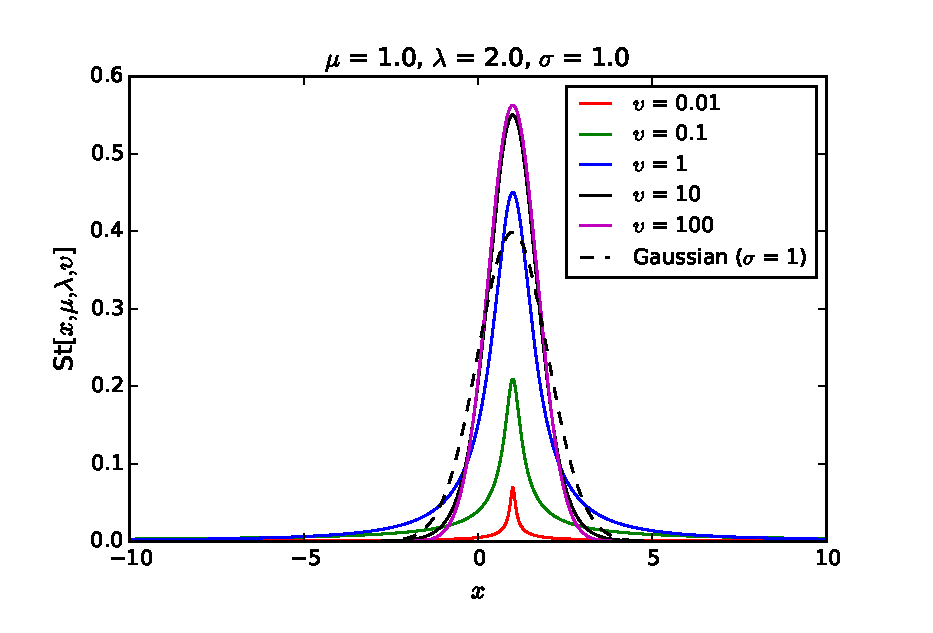
\includegraphics[width=0.8\textwidth]{./figures/3f2.eps}
 \caption{Student's t-distribution.}
 \label{fig:3f2}
\end{figure}
\begin{figure}[htb]
 \centering
 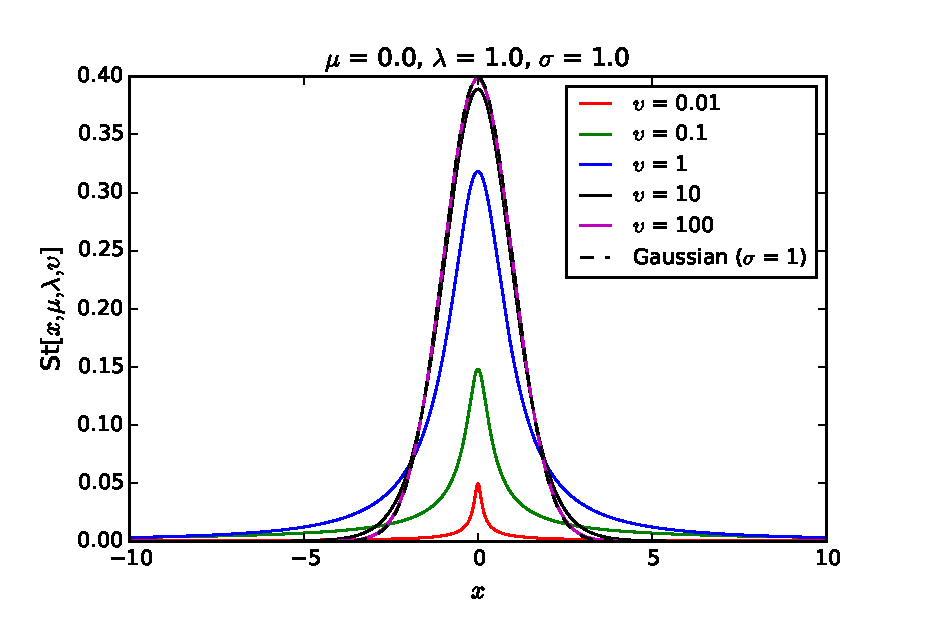
\includegraphics[width=0.8\textwidth]{./figures/3f1.eps}
 \caption{Student's t-distribution for $\mu=0$ and $\lambda=1$.}
 \label{fig:3f1}
\end{figure}

\cleardoublepage
\subsection*{Exercise \#04}
The provided data was modeled as a mixture of Gaussians as depicted in Figure \ref{fig:4f1}. The red curve is the distribution probability generated by mixing 6 normal distributions with $\sigma=1$ and $\mu \in \{-10, -6, 12, 15, 19, 50\}$. Note, however, that this model is overfit, since the provided data might not represent the whole data population. 
\begin{figure}[htb]
 \centering
 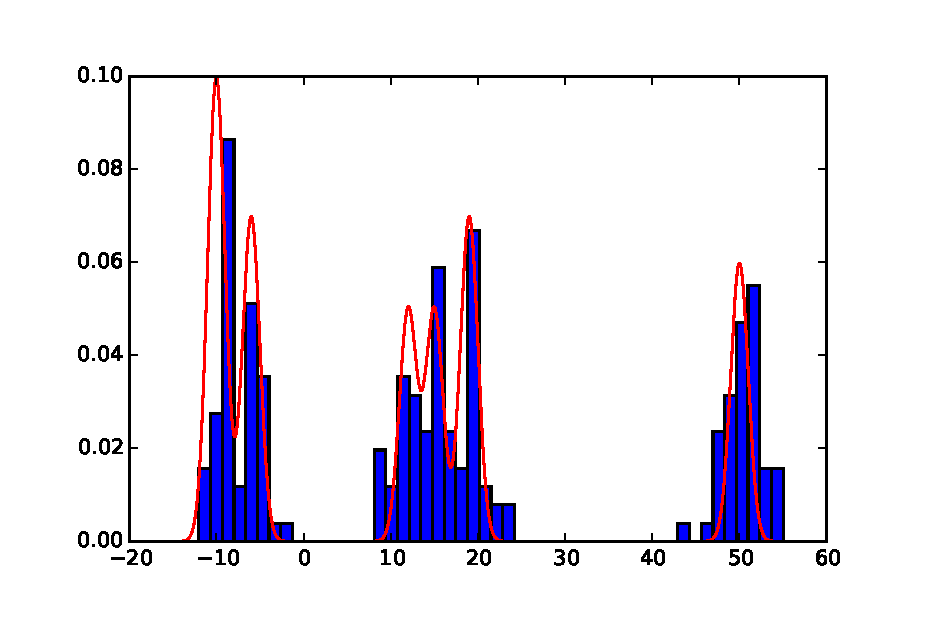
\includegraphics[width=0.8\textwidth]{./figures/4f1.eps}
 \caption{Estimated probability density function provided by the mixture of Gaussians model.}
 \label{fig:4f1}
\end{figure}

\cleardoublepage
\subsection*{Exercise \#05}
Kernel density estimators were used in this exercise to estimate the density function of the provided data. The estimates provided by a Gaussian and a rectangular kernel for different window length $h$ are depicted in Figures \ref{fig:5f1} and \ref{fig:5f2}, respectively. As $h$ increases, the estimated curve becomes smoother. 
\begin{figure}[htb]
 \centering
 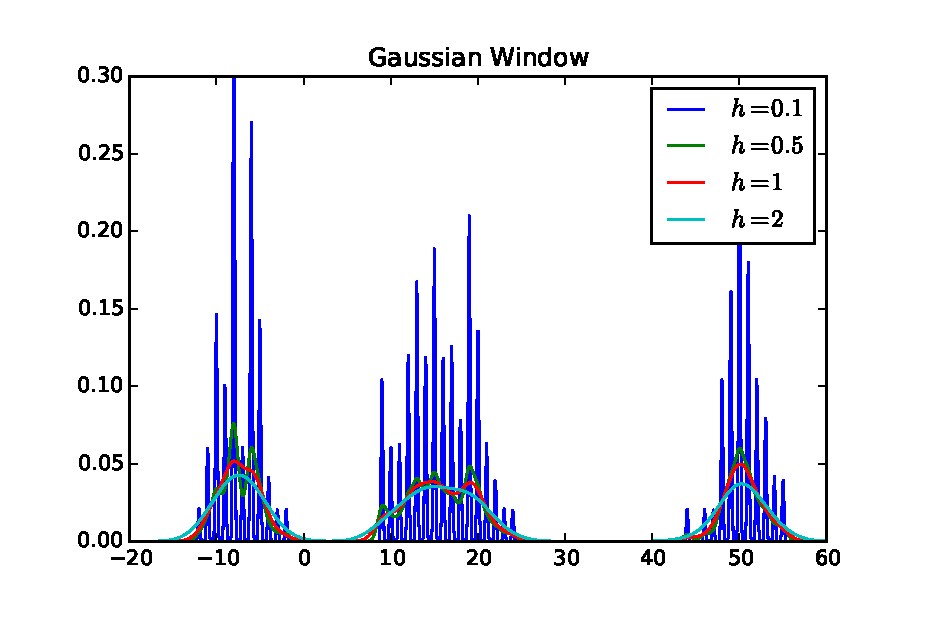
\includegraphics[width=0.7\textwidth]{./figures/5f1.eps}
 \caption{Probability density curve estimated using Gaussian kernel.}
 \label{fig:5f1}
\end{figure}
\begin{figure}[htb]
 \centering
 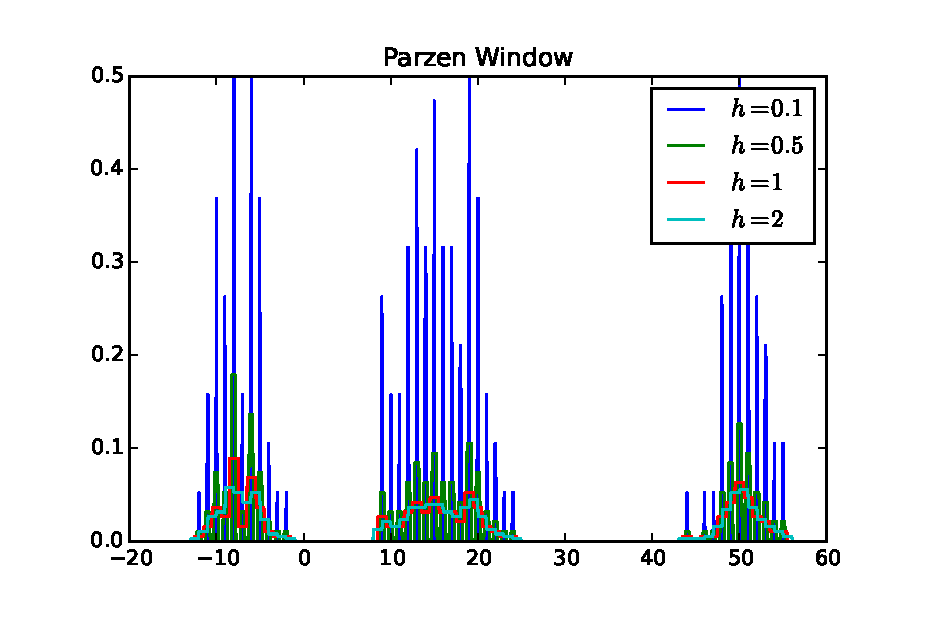
\includegraphics[width=0.7\textwidth]{./figures/5f2.eps}
 \caption{Probability density curve estimated using Parzen kernel.}
 \label{fig:5f2}
\end{figure}

\cleardoublepage
\subsection*{Exercise \#06}

\paragraph{Identity basis function} The mean square error (MSE) obtained in the training and test stages are
\begin{verbatim}
 MSE [learning]:  1.03728146352
 MSE [test]:  1.10867871973
\end{verbatim}
The predicted output is shown in Figure \ref{fig:6f1}. In this case, the predictions were not correct in general, resulting in a large MSE value.

\paragraph{Gaussian basis function} In the evaluation stage, the MSE and the norm of the regression coefficents vector $\mb{w}$ were plotted in function of the number of basis function $M$ in Figures \ref{fig:6f2} and \ref{fig:6f3}, respectively. It was observed that $\|\mb{w}\|_2$ grows greatly with $M$, indicating that the model is overfit for large $M$. Additionally, it could be seen that the MSE did not decrease for values larger than 40. The number of basis function was set to $M=45$. 

The MSE obtained in the training and test stages were
\begin{verbatim}
MSE [learning]:  0.064172108973
MSE [test]:  0.05952864372
\end{verbatim}
The predicted values are compared to the actual values in Figure \ref{fig:6f4}. It can be seen that the predictions were accurate in general, as indicated by the low MSE values.

\begin{figure}[htb]
 \centering
 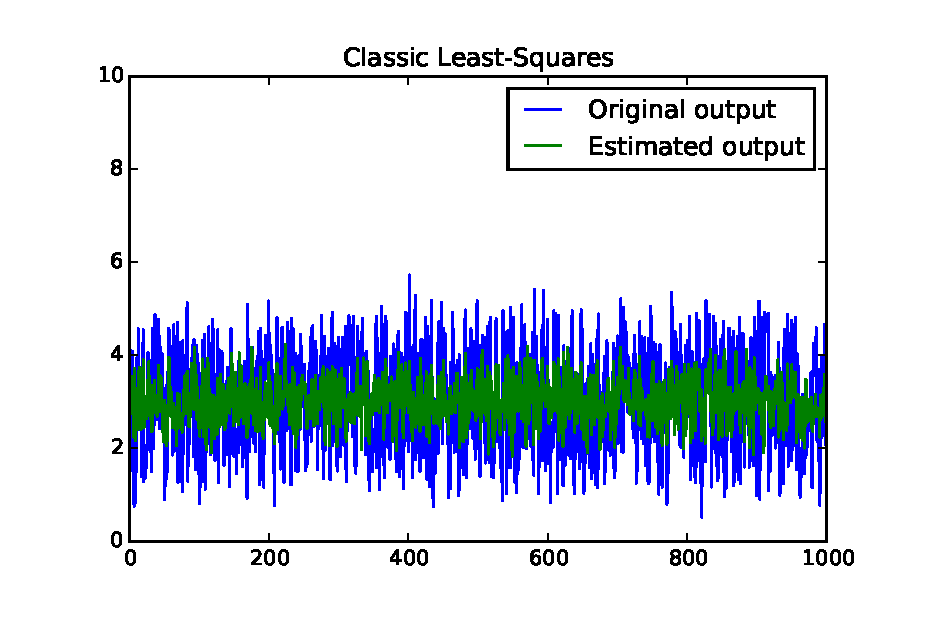
\includegraphics[width=0.7\textwidth]{./figures/6f1.eps}
 \caption{Predicted output using identity basis function.}
 \label{fig:6f1}
\end{figure}
\begin{figure}[htb]
 \centering
 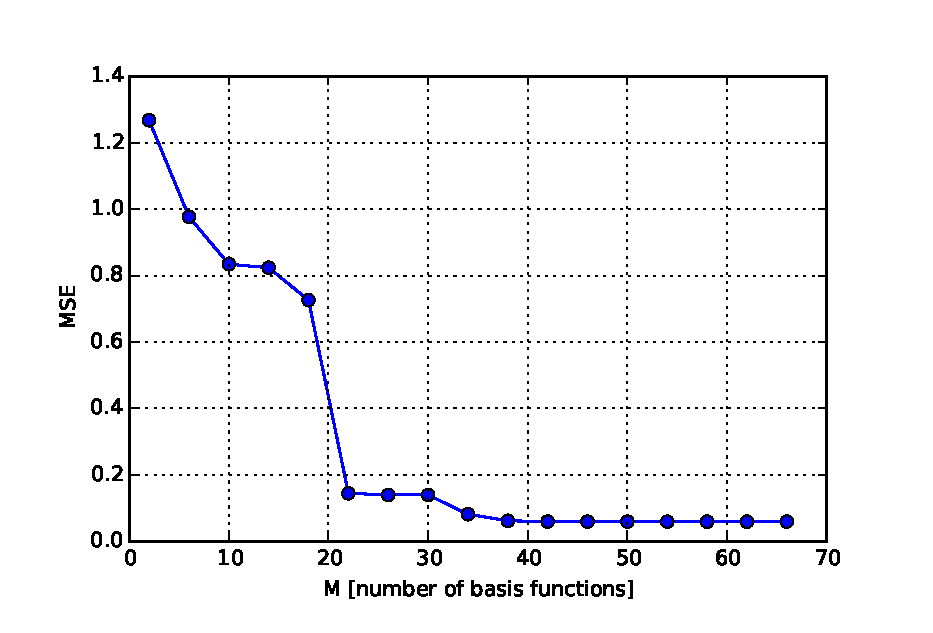
\includegraphics[width=0.7\textwidth]{./figures/6f2.eps}
 \caption{MSE vs. number of basis functions ($M$).}
 \label{fig:6f2}
\end{figure}
\begin{figure}[htb]
 \centering
 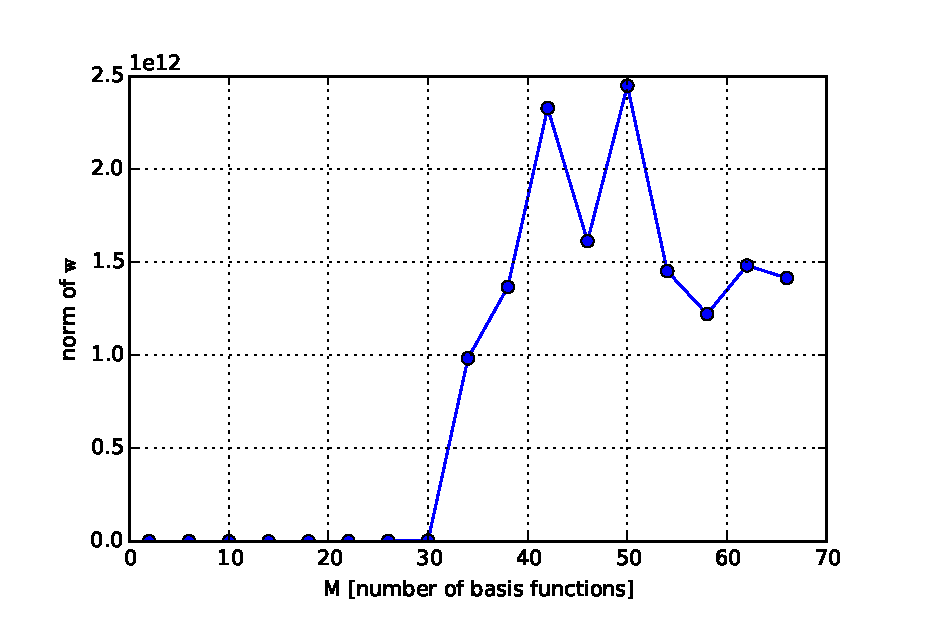
\includegraphics[width=0.7\textwidth]{./figures/6f3.eps}
 \caption{norm of $\mb{w}$ vs. number of basis functions ($M$).}
 \label{fig:6f3}
\end{figure}
\begin{figure}[htb]
 \centering
 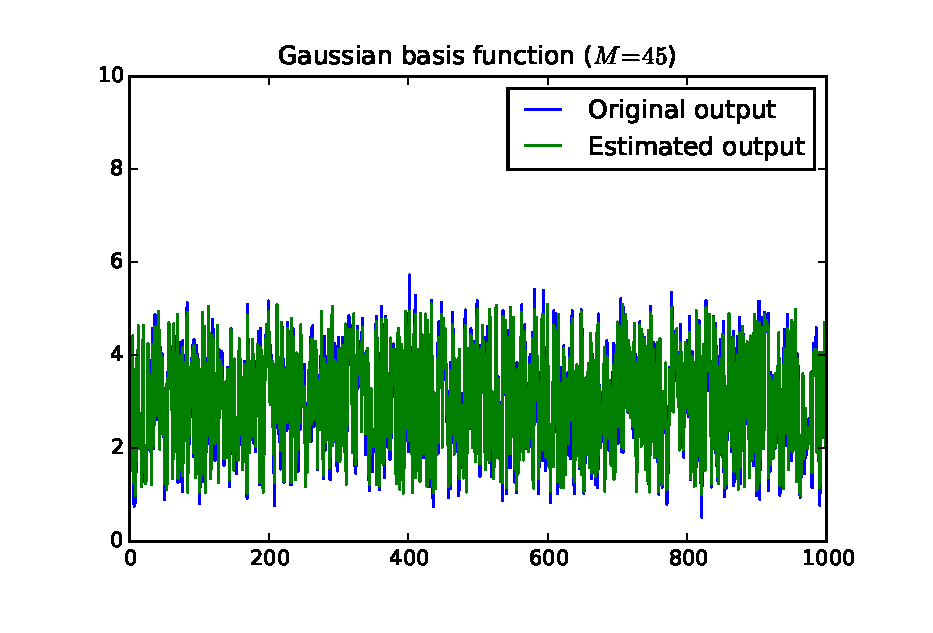
\includegraphics[width=0.7\textwidth]{./figures/6f4.eps}
 \caption{Predicted output using Gaussian basis functions.}
 \label{fig:6f4}
\end{figure}

\cleardoublepage
\subsection*{Exercise \#07}
In the previous exercise, the norm of $\mb{w}$ grew greatly with the number of basis functions, indicating that the model may be overfit. By considering a regularization component that limits $\|\mb{w}\|_2$ in the objective function, the overfitting is reduced. In this exercise, the effect of regularization was analyzed by changing the values of the regularization factor $\lambda$. The MSE did not improve with the different values of the regularization parameter, as depicted in Figures \ref{fig:7f1}. However, in Figure \ref{fig:7f2} it could be seen that the norm of $\mb{w}$ decreased as $\lambda$ grew. In Figure \ref{fig:7f3}, the predictions made with $\lambda=1$ are compared to the actual values. The MSE in the training and test stages for this $\lambda$ were:
\begin{verbatim}
 MSE [learning]:  1.04197164446
 MSE [test]:  1.11608842949
\end{verbatim}


\begin{figure}[htb]
 \centering
 \includegraphics[width=0.7\textwidth]{./figures/7f1.eps}
 \caption{Probability density curve estimated using Parzen kernel.}
 \label{fig:7f1}
\end{figure}
\begin{figure}[htb]
 \centering
 \includegraphics[width=0.7\textwidth]{./figures/7f2.eps}
 \caption{Probability density curve estimated using Parzen kernel.}
 \label{fig:7f2}
\end{figure}
\begin{figure}[htb]
 \centering
 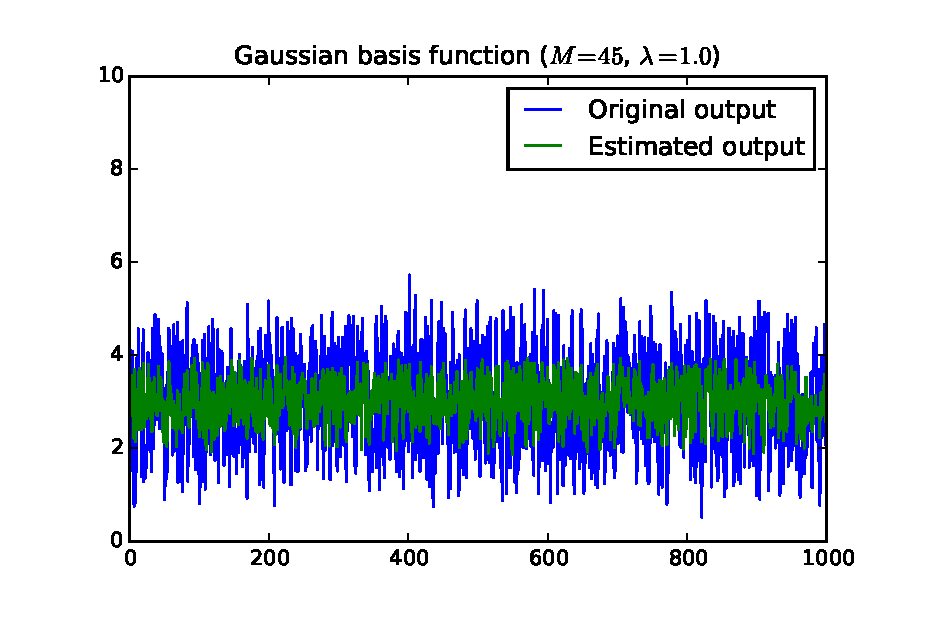
\includegraphics[width=0.7\textwidth]{./figures/7f3.eps}
 \caption{Probability density curve estimated using Parzen kernel.}
 \label{fig:7f3}
\end{figure}

\cleardoublepage
\subsection*{Exercise \#08}
In this exercise a linear model was proposed to predict the provided data. The parameters of this model were estimated using a Bayesian linear regression method in which the posterior function was a zero-mean isotropic Gaussian distribution. In this case, the maximum posterior weight vector is equal to its mean vector. The estimated mean vector from the provided data is
\begin{verbatim}
mn:
[[-0.06587564]
 [ 0.4999401 ]]
\end{verbatim}
and the predicted curve is depicted in Figure \ref{fig:8f1}.
\begin{figure}[htb]
 \centering
 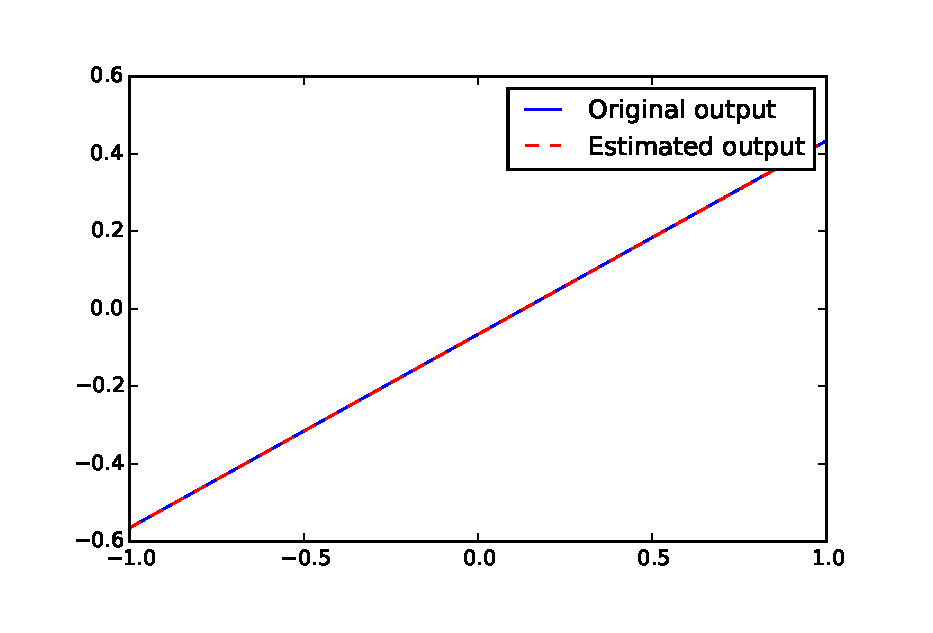
\includegraphics[width=0.7\textwidth]{./figures/8f1.eps}
 \caption{Bayesian linear regression.}
 \label{fig:8f1}
\end{figure}
\end{document}

